\documentclass[tikz]{standalone}
\usepackage[utf8]{inputenc}
\usepackage{tikz}
\usepackage{xcolor}
\usepackage{xcolor}
\usepackage{scalerel}
\usepackage{graphicx}
\usetikzlibrary{decorations.pathreplacing,calligraphy}
\usepackage{amsmath,amssymb,amsfonts}
\usepackage{dsfont}

\definecolor{MyGreen}{RGB}{34,139,34}

\begin{document}






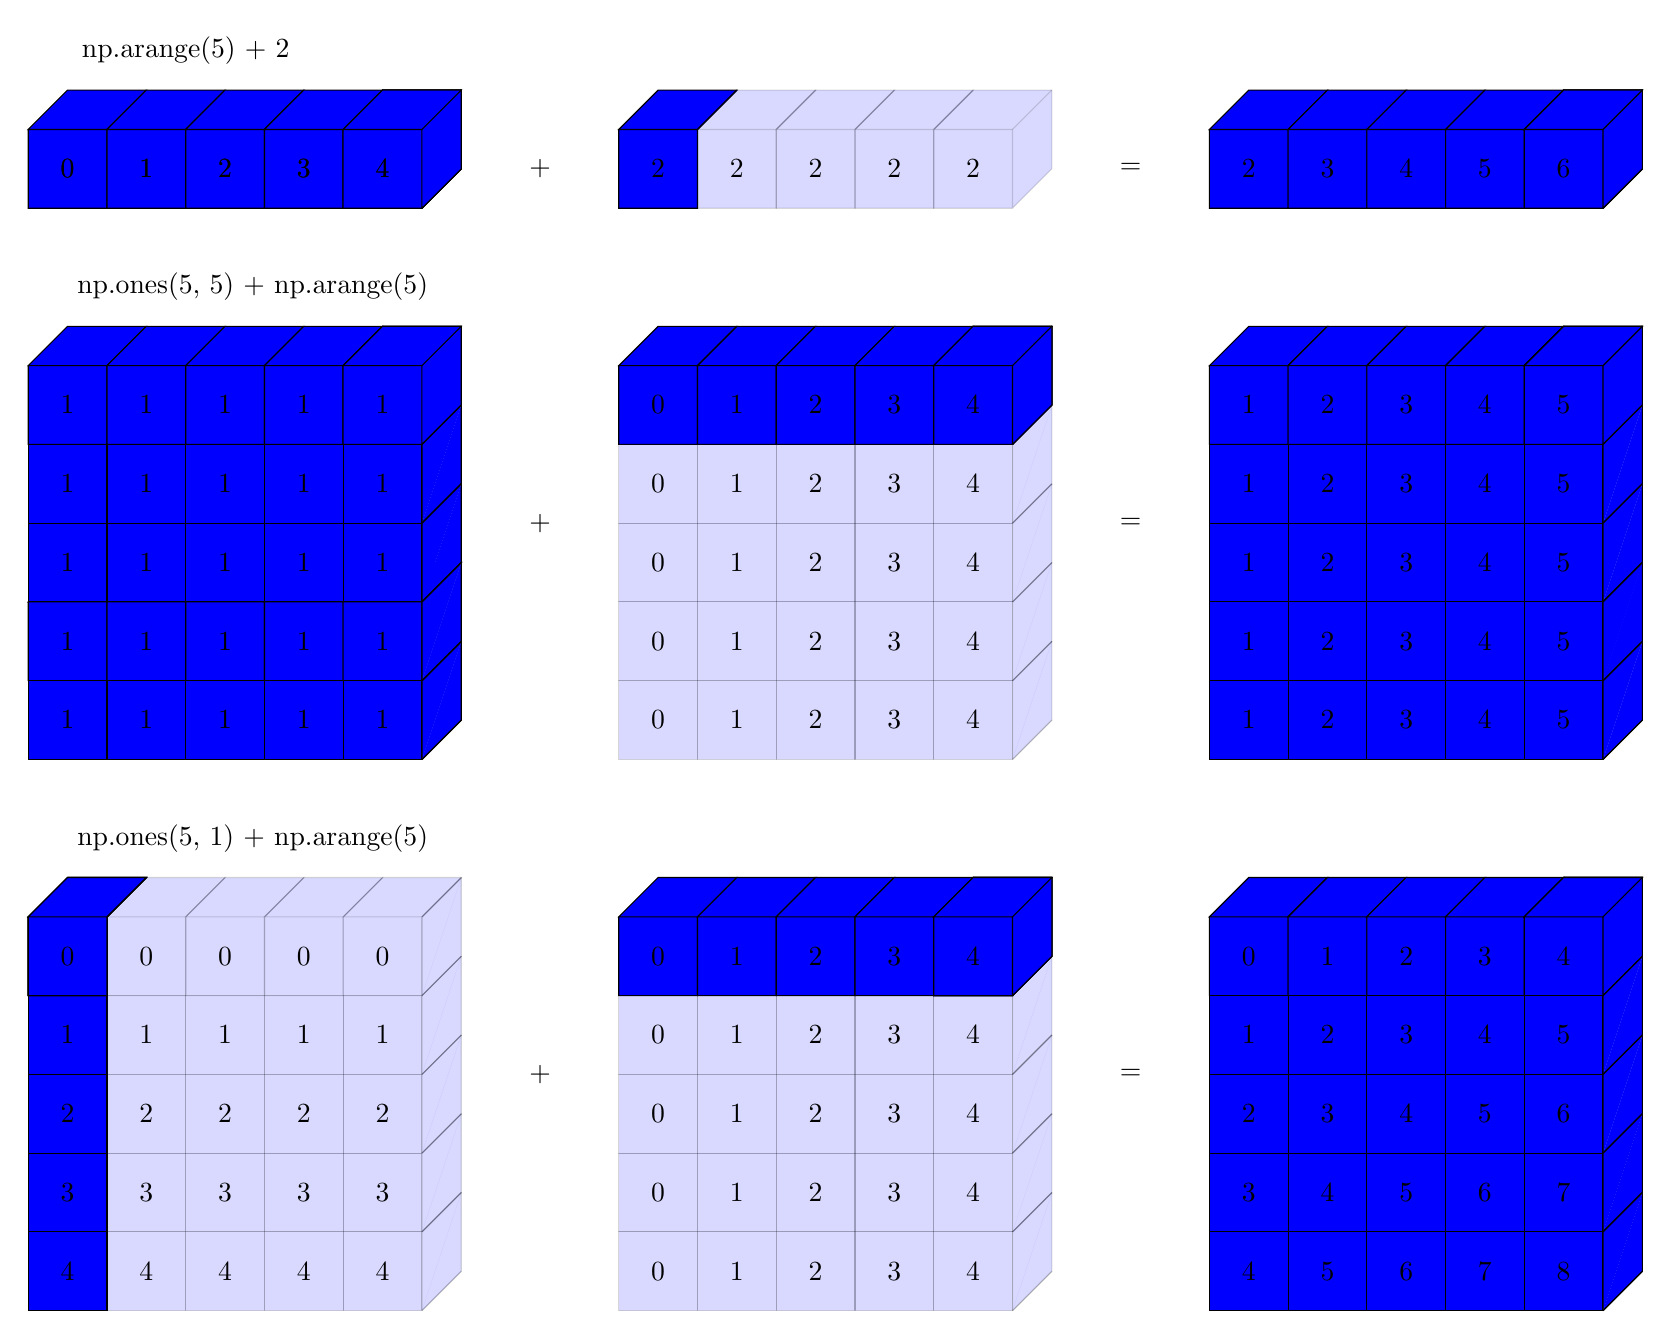
\begin{tikzpicture}[z={(0.5,0.5)}]
\node[align=left] at (3,2) {\text{{\fontfamily{cmt}\selectfont np.arange(5)} + 2}};
\def\cubesAmount{5}
\foreach \i in {1,...,\cubesAmount}{
    \draw[fill = blue] (\i,0,0) rectangle +(1,1,0) -- ++(0,1,0) -- ++(0,0,1) -- ++(1,0,0) edge +(0,0,-1)  -- ++(0,0,-1);
    \draw[fill = blue] (5,0,0) rectangle +(1,1,0) -- ++(0,1,0) -- ++(0,0,1) -- ++(1,0,0) edge +(0,0,-1) -- ++(0,-1,0) -- ++(0,0,-1);
    \ifnum\i<\cubesAmount
       ;
    \fi
}
\node[align=left] at (1.5,0.5) {0};
\node[align=left] at (2.5,0.5) {1};
\node[align=left] at (3.5,0.5) {2};
\node[align=left] at (4.5,0.5) {3};
\node[align=left] at (5.5,0.5) {4};

\node[align=left] at (7.5,0.5) {+};

\draw[fill = blue] (7.5 + 1,0,0) rectangle +(1,1,0) -- ++(0,1,0) -- ++(0,0,1) -- ++(1,0,0) edge +(0,0,-1)  -- ++(0,0,-1);
 
\def\cubesAmount{3}
\foreach \i in {1,...,\cubesAmount}{
    \draw[fill = blue, opacity=0.15] (8.5 + \i,0,0) rectangle +(1,1,0) -- ++(0,1,0) -- ++(0,0,1) -- ++(1,0,0) edge +(0,0,-1)  -- ++(0,0,-1);
    \ifnum\i<\cubesAmount
       ;
    \fi
}

\draw[fill = blue, opacity=0.15] (12.5,0,0) rectangle +(1,1,0) -- ++(0,1,0) -- ++(0,0,1) -- ++(1,0,0) edge +(0,0,-1) -- ++(0,-1,0) -- ++(0,0,-1);

\node[align=left] at (9,0.5) {2};
\node[align=left] at (10,0.5) {2};
\node[align=left] at (11,0.5) {2};
\node[align=left] at (12,0.5) {2};
\node[align=left] at (13,0.5) {2};
%\node[align=left] at (14,0.5) {2};

\node[align=left] at (15,0.5) {=};

\def\cubesAmount{5}
\foreach \i in {1,...,\cubesAmount}{
    \draw[fill = blue] (15 + \i,0,0) rectangle +(1,1,0) -- ++(0,1,0) -- ++(0,0,1) -- ++(1,0,0) edge +(0,0,-1)  -- ++(0,0,-1);
    \draw[fill = blue] (20,0,0) rectangle +(1,1,0) -- ++(0,1,0) -- ++(0,0,1) -- ++(1,0,0) edge +(0,0,-1) -- ++(0,-1,0) -- ++(0,0,-1);
    \ifnum\i<\cubesAmount
       ;
    \fi
}
\node[align=left] at (16.5,0.5) {2};
\node[align=left] at (17.5,0.5) {3};
\node[align=left] at (18.5,0.5) {4};
\node[align=left] at (19.5,0.5) {5};
\node[align=left] at (20.5,0.5) {6};








\node[align=left] at (3.85,-1) {\text{{\fontfamily{cmt}\selectfont np.ones(5, 5)} + np.arange(5)}};
\def\cubesAmount{5}
\foreach \i in {1,...,\cubesAmount}{
    \draw[fill = blue] (\i,-3,0) rectangle +(1,1,0) -- ++(0,1,0) -- ++(0,0,1) -- ++(1,0,0) edge +(0,0,-1)  -- ++(0,0,-1);
    \draw[fill = blue] (\i,-6,0) rectangle +(1,1,0) -- ++(0,1,0) -- ++(0,0,1) -- ++(1,0,0) edge +(0,0,-1)  -- ++(0,0,-1);
    \draw[fill = blue] (5,-3,0) rectangle +(1,1,0) -- ++(0,1,0) -- ++(0,0,1) -- ++(1,0,0) edge +(0,0,-1) -- ++(0,-1,0) -- ++(0,0,-1);
    \draw[fill = blue] (\i,-4,0) rectangle +(1,1,0) -- ++(0,1,0);
    \draw[fill = blue] (\i,-5,0) rectangle +(1,1,0) -- ++(0,1,0);
   %\draw[fill = blue] (7,-2,0) edge +(0,0,-1) -- ++(0,-1,0) -- ++(0,0,-1);
    \draw[fill = blue] (\i,-7,0) rectangle +(1,1,0) -- ++(0,1,0) ;
    \ifnum\i<\cubesAmount
       ;
    \fi
}

\draw[fill = blue] (6.5, -2.5,0) edge +(0,0,-1) -- ++(0,-1,0) -- ++(0,0,-1);
\draw[fill = blue, rotate=180] (-6.001, 4.001,0) edge +(0,0,-1) -- ++(0,-1,0) -- ++(0,0,-1);


\draw[fill = blue] (6.5, -3.5,0) edge +(0,0,-1) -- ++(0,-1,0) -- ++(0,0,-1);
\draw[fill = blue, rotate=180] (-6.001, 5.001,0) edge +(0,0,-1) -- ++(0,-1,0) -- ++(0,0,-1);

\draw[fill = blue] (6.5, -5.5,0) edge +(0,0,-1) -- ++(0,-1,0) -- ++(0,0,-1);
\draw[fill = blue, rotate=180] (-6.001, 7.001,0) edge +(0,0,-1) -- ++(0,-1,0) -- ++(0,0,-1);

\draw[fill = blue] (6.5, -4.5,0) edge +(0,0,-1) -- ++(0,-1,0) -- ++(0,0,-1);
\draw[fill = blue, rotate=180] (-6.001, 6.001,0) edge +(0,0,-1) -- ++(0,-1,0) -- ++(0,0,-1);

\node[align=left] at (1.5,0.5) {0};
\node[align=left] at (2.5,0.5) {1};
\node[align=left] at (3.5,0.5) {2};
\node[align=left] at (4.5,0.5) {3};
\node[align=left] at (5.5,0.5) {4};

\node[align=left] at (7.5,-4) {+};

\node[align=left] at (1.5,-2.5) {1};
\node[align=left] at (2.5,-2.5) {1};
\node[align=left] at (3.5,-2.5) {1};
\node[align=left] at (4.5,-2.5) {1};
\node[align=left] at (5.5,-2.5) {1};

\node[align=left] at (1.5,-3.5) {1};
\node[align=left] at (2.5,-3.5) {1};
\node[align=left] at (3.5,-3.5) {1};
\node[align=left] at (4.5,-3.5) {1};
\node[align=left] at (5.5,-3.5) {1};

\node[align=left] at (1.5,-4.5) {1};
\node[align=left] at (2.5,-4.5) {1};
\node[align=left] at (3.5,-4.5) {1};
\node[align=left] at (4.5,-4.5) {1};
\node[align=left] at (5.5,-4.5) {1};

\node[align=left] at (1.5,-5.5) {1};
\node[align=left] at (2.5,-5.5) {1};
\node[align=left] at (3.5,-5.5) {1};
\node[align=left] at (4.5,-5.5) {1};
\node[align=left] at (5.5,-5.5) {1};

\node[align=left] at (1.5,-6.5) {1};
\node[align=left] at (2.5,-6.5) {1};
\node[align=left] at (3.5,-6.5) {1};
\node[align=left] at (4.5,-6.5) {1};
\node[align=left] at (5.5,-6.5) {1};

\def\cubesAmount{5}
\foreach \i in {1,...,\cubesAmount}{
    \draw[fill = blue] (\i+ 7.5,-3,0) rectangle +(1,1,0) -- ++(0,1,0) -- ++(0,0,1) -- ++(1,0,0) edge +(0,0,-1)  -- ++(0,0,-1);
    \draw[fill = blue] (12.5,-3,0) rectangle +(1,1,0) -- ++(0,1,0) -- ++(0,0,1) -- ++(1,0,0) edge +(0,0,-1) -- ++(0,-1,0) -- ++(0,0,-1);
    \draw[fill = blue, opacity=0.15] (\i +7.5,-4,0) rectangle +(1,1,0) -- ++(0,1,0);
     \draw[fill = blue, opacity=0.15] (\i +7.5,-6,0) rectangle +(1,1,0) -- ++(0,1,0);
      \draw[fill = blue, opacity=0.15] (\i +7.5,-7,0) rectangle +(1,1,0) -- ++(0,1,0);
   %\draw[fill = blue] (7,-2,0) edge +(0,0,-1) -- ++(0,-1,0) -- ++(0,0,-1);
    \draw[fill = blue, opacity=0.15] (\i+7.5,-5,0) rectangle +(1,1,0) -- ++(0,1,0) ;
    \ifnum\i<\cubesAmount
       ;
    \fi
}

\draw[fill = blue, opacity=0.15] (14, -2.5,0) edge +(0,0,-1) -- ++(0,-1,0) -- ++(0,0,-1);
\draw[fill = blue, rotate=180, opacity=0.15] (-13.501, 4.001,0) edge +(0,0,-1) -- ++(0,-1,0) -- ++(0,0,-1);


\draw[fill = blue, opacity=0.15] (14, -3.5,0) edge +(0,0,-1) -- ++(0,-1,0) -- ++(0,0,-1);
\draw[fill = blue, rotate=180, opacity=0.15] (-13.501, 5.001,0) edge +(0,0,-1) -- ++(0,-1,0) -- ++(0,0,-1);

\draw[fill = blue, opacity=0.15] (14, -4.5,0) edge +(0,0,-1) -- ++(0,-1,0) -- ++(0,0,-1);
\draw[fill = blue, rotate=180, opacity=0.15] (-13.501, 6.001,0) edge +(0,0,-1) -- ++(0,-1,0) -- ++(0,0,-1);

\draw[fill = blue, opacity=0.15] (14, -5.5,0) edge +(0,0,-1) -- ++(0,-1,0) -- ++(0,0,-1);
\draw[fill = blue, rotate=180, opacity=0.15] (-13.501, 7.001,0) edge +(0,0,-1) -- ++(0,-1,0) -- ++(0,0,-1);

\node[align=left] at (9,-2.5) {0};
\node[align=left] at (10,-2.5) {1};
\node[align=left] at (11,-2.5) {2};
\node[align=left] at (12,-2.5) {3};
\node[align=left] at (13,-2.5) {4};

\node[align=left] at (9,-3.5) {0};
\node[align=left] at (10,-3.5) {1};
\node[align=left] at (11,-3.5) {2};
\node[align=left] at (12,-3.5) {3};
\node[align=left] at (13,-3.5) {4};

\node[align=left] at (9,-4.5) {0};
\node[align=left] at (10,-4.5) {1};
\node[align=left] at (11,-4.5) {2};
\node[align=left] at (12,-4.5) {3};
\node[align=left] at (13,-4.5) {4};

\node[align=left] at (9,-5.5) {0};
\node[align=left] at (10,-5.5) {1};
\node[align=left] at (11,-5.5) {2};
\node[align=left] at (12,-5.5) {3};
\node[align=left] at (13,-5.5) {4};

\node[align=left] at (9,-6.5) {0};
\node[align=left] at (10,-6.5) {1};
\node[align=left] at (11,-6.5) {2};
\node[align=left] at (12,-6.5) {3};
\node[align=left] at (13,-6.5) {4};

\node[align=left] at (15,-4) {=};

\def\cubesAmount{5}
\foreach \i in {1,...,\cubesAmount}{
    \draw[fill = blue] (\i+15,-3,0) rectangle +(1,1,0) -- ++(0,1,0) -- ++(0,0,1) -- ++(1,0,0) edge +(0,0,-1)  -- ++(0,0,-1);
    \draw[fill = blue] (20,-3,0) rectangle +(1,1,0) -- ++(0,1,0) -- ++(0,0,1) -- ++(1,0,0) edge +(0,0,-1) -- ++(0,-1,0) -- ++(0,0,-1);
    \draw[fill = blue] (\i+15,-4,0) rectangle +(1,1,0) -- ++(0,1,0);
     \draw[fill = blue] (\i+15,-6,0) rectangle +(1,1,0) -- ++(0,1,0);
      \draw[fill = blue] (\i+15,-7,0) rectangle +(1,1,0) -- ++(0,1,0);
   %\draw[fill = blue] (7,-2,0) edge +(0,0,-1) -- ++(0,-1,0) -- ++(0,0,-1);
    \draw[fill = blue] (\i+15,-5,0) rectangle +(1,1,0) -- ++(0,1,0) ;
    \ifnum\i<\cubesAmount
       ;
    \fi
}

\draw[fill = blue] (21.5, -2.5,0) edge +(0,0,-1) -- ++(0,-1,0) -- ++(0,0,-1);
\draw[fill = blue, rotate=180] (-21.001, 4.001,0) edge +(0,0,-1) -- ++(0,-1,0) -- ++(0,0,-1);


\draw[fill = blue] (21.5, -3.5,0) edge +(0,0,-1) -- ++(0,-1,0) -- ++(0,0,-1);
\draw[fill = blue, rotate=180] (-21.001, 5.001,0) edge +(0,0,-1) -- ++(0,-1,0) -- ++(0,0,-1);

\draw[fill = blue] (21.5, -4.5,0) edge +(0,0,-1) -- ++(0,-1,0) -- ++(0,0,-1);
\draw[fill = blue, rotate=180] (-21.001, 6.001,0) edge +(0,0,-1) -- ++(0,-1,0) -- ++(0,0,-1);

\draw[fill = blue] (21.5, -5.5,0) edge +(0,0,-1) -- ++(0,-1,0) -- ++(0,0,-1);
\draw[fill = blue, rotate=180] (-21.001, 7.001,0) edge +(0,0,-1) -- ++(0,-1,0) -- ++(0,0,-1);

\node[align=left] at (16.5,-2.5) {1};
\node[align=left] at (17.5,-2.5) {2};
\node[align=left] at (18.5,-2.5) {3};
\node[align=left] at (19.5,-2.5) {4};
\node[align=left] at (20.5,-2.5) {5};

\node[align=left] at (16.5,-3.5) {1};
\node[align=left] at (17.5,-3.5) {2};
\node[align=left] at (18.5,-3.5) {3};
\node[align=left] at (19.5,-3.5) {4};
\node[align=left] at (20.5,-3.5) {5};

\node[align=left] at (16.5,-4.5) {1};
\node[align=left] at (17.5,-4.5) {2};
\node[align=left] at (18.5,-4.5) {3};
\node[align=left] at (19.5,-4.5) {4};
\node[align=left] at (20.5,-4.5) {5};

\node[align=left] at (16.5,-5.5) {1};
\node[align=left] at (17.5,-5.5) {2};
\node[align=left] at (18.5,-5.5) {3};
\node[align=left] at (19.5,-5.5) {4};
\node[align=left] at (20.5,-5.5) {5};

\node[align=left] at (16.5,-6.5) {1};
\node[align=left] at (17.5,-6.5) {2};
\node[align=left] at (18.5,-6.5) {3};
\node[align=left] at (19.5,-6.5) {4};
\node[align=left] at (20.5,-6.5) {5};

\node[align=left] at (3.85,-8) {\text{{\fontfamily{cmt}\selectfont np.ones(5, 1)} + np.arange(5)}};
\def\cubesAmount{4}
\foreach \i in {1,...,\cubesAmount}{
    %\draw[fill = blue] (1,-12,0) rectangle +(1,1,0) -- ++(0,1,0) -- ++(0,0,1) -- ++(1,0,0) edge +(0,0,-1)  -- ++(0,0,-1);
    \draw[fill = blue] (1,-10,0) rectangle +(1,1,0) -- ++(0,1,0) -- ++(0,0,1) -- ++(1,0,0) edge +(0,0,-1)  -- ++(0,0,-1);
    \draw[fill = blue] (1,-10-\i,0) rectangle +(1,1,0) -- ++(0,1,0);
    \draw[fill = blue, opacity = 0.15] (\i + 1,-10,0) rectangle +(1,1,0) -- ++(0,1,0) -- ++(0,0,1) -- ++(1,0,0) edge +(0,0,-1)  -- ++(0,0,-1);
    %\draw[fill = blue, opacity = 0.15] (5,-8,0) rectangle +(1,1,0) -- ++(0,1,0) ;
    \draw[fill = blue, opacity = 0.15] (\i + 1,-11,0) rectangle +(1,1,0) -- ++(0,1,0);
    \draw[fill = blue, opacity = 0.15] (\i + 1,-12,0) rectangle +(1,1,0) -- ++(0,1,0);
    \draw[fill = blue, opacity = 0.15] (\i + 1,-13,0) rectangle +(1,1,0) -- ++(0,1,0);
    \draw[fill = blue, opacity = 0.15] (\i + 1,-14,0) rectangle +(1,1,0) -- ++(0,1,0);
   %\draw[fill = blue] (7,-2,0) edge +(0,0,-1) -- ++(0,-1,0) -- ++(0,0,-1);
    %\draw[fill = blue, opacity = 0.15] (\i + 1,-8,0) rectangle +(1,1,0) -- ++(0,1,0) ;
    \ifnum\i<\cubesAmount
       ;
    \fi
}

\draw[fill = blue, opacity = 0.15] (6.5, -9.5,0) edge +(0,0,-1) -- ++(0,-1,0) -- ++(0,0,-1);
\draw[fill = blue, opacity = 0.15] (6.5, -8.5,0) edge +(0,0,-1) -- ++(0,-1,0) -- ++(0,0,-1);


\draw[fill = blue, rotate=180, opacity = 0.15] (-6.001, 11.001,0) edge +(0,0,-1) -- ++(0,-1,0) -- ++(0,0,-1);
\draw[fill = blue, rotate=180, opacity = 0.15] (-6.001, 10.001,0) edge +(0,0,-1) -- ++(0,-1,0) -- ++(0,0,-1);

\draw[fill = blue, rotate=180, opacity = 0.15] (-6.001, 12.001,0) edge +(0,0,-1) -- ++(0,-1,0) -- ++(0,0,-1);
\draw[fill = blue, opacity = 0.15] (6.5, -10.5,0) edge +(0,0,-1) -- ++(0,-1,0) -- ++(0,0,-1);

\draw[fill = blue, rotate=180, opacity = 0.15] (-6.001, 13.001,0) edge +(0,0,-1) -- ++(0,-1,0) -- ++(0,0,-1);
\draw[fill = blue, opacity = 0.15] (6.5, -11.5,0) edge +(0,0,-1) -- ++(0,-1,0) -- ++(0,0,-1);

\draw[fill = blue, rotate=180, opacity = 0.15] (-6.001, 14.001,0) edge +(0,0,-1) -- ++(0,-1,0) -- ++(0,0,-1);
\draw[fill = blue, opacity = 0.15] (6.5, -12.5,0) edge +(0,0,-1) -- ++(0,-1,0) -- ++(0,0,-1);


\node[align=left] at (7.5,-11) {+};

\node[align=left] at (1.5,-9.5) {0};
\node[align=left] at (2.5,-9.5) {0};
\node[align=left] at (3.5,-9.5) {0};
\node[align=left] at (4.5,-9.5) {0};
\node[align=left] at (5.5,-9.5) {0};

\node[align=left] at (1.5,-10.5) {1};
\node[align=left] at (2.5,-10.5) {1};
\node[align=left] at (3.5,-10.5) {1};
\node[align=left] at (4.5,-10.5) {1};
\node[align=left] at (5.5,-10.5) {1};

\node[align=left] at (1.5,-11.5) {2};
\node[align=left] at (2.5,-11.5) {2};
\node[align=left] at (3.5,-11.5) {2};
\node[align=left] at (4.5,-11.5) {2};
\node[align=left] at (5.5,-11.5) {2};

\node[align=left] at (1.5,-12.5) {3};
\node[align=left] at (2.5,-12.5) {3};
\node[align=left] at (3.5,-12.5) {3};
\node[align=left] at (4.5,-12.5) {3};
\node[align=left] at (5.5,-12.5) {3};

\node[align=left] at (1.5,-13.5) {4};
\node[align=left] at (2.5,-13.5) {4};
\node[align=left] at (3.5,-13.5) {4};
\node[align=left] at (4.5,-13.5) {4};
\node[align=left] at (5.5,-13.5) {4};



\def\cubesAmount{5}
\foreach \i in {1,...,\cubesAmount}{
    \draw[fill = blue] (\i+ 7.5,-10,0) rectangle +(1,1,0) -- ++(0,1,0) -- ++(0,0,1) -- ++(1,0,0) edge +(0,0,-1)  -- ++(0,0,-1);
    \draw[fill = blue] (12.5,-10,0) rectangle +(1,1,0) -- ++(0,1,0) -- ++(0,0,1) -- ++(1,0,0) edge +(0,0,-1) -- ++(0,-1,0) -- ++(0,0,-1);
    \draw[fill = blue, opacity=0.15] (\i +7.5,-11,0) rectangle +(1,1,0) -- ++(0,1,0);
     \draw[fill = blue, opacity=0.15] (\i +7.5,-12,0) rectangle +(1,1,0) -- ++(0,1,0);
      \draw[fill = blue, opacity=0.15] (\i +7.5,-13,0) rectangle +(1,1,0) -- ++(0,1,0);
   %\draw[fill = blue] (7,-2,0) edge +(0,0,-1) -- ++(0,-1,0) -- ++(0,0,-1);
    \draw[fill = blue, opacity=0.15] (\i+7.5,-14,0) rectangle +(1,1,0) -- ++(0,1,0) ;
    \ifnum\i<\cubesAmount
       ;
    \fi
}

\draw[fill = blue, opacity=0.15] (14, -9.5,0) edge +(0,0,-1) -- ++(0,-1,0) -- ++(0,0,-1);
\draw[fill = blue, rotate=180, opacity=0.15] (-13.501, 11.001,0) edge +(0,0,-1) -- ++(0,-1,0) -- ++(0,0,-1);


\draw[fill = blue, opacity=0.15] (14, -10.5,0) edge +(0,0,-1) -- ++(0,-1,0) -- ++(0,0,-1);
\draw[fill = blue, rotate=180, opacity=0.15] (-13.501, 12.001,0) edge +(0,0,-1) -- ++(0,-1,0) -- ++(0,0,-1);

\draw[fill = blue, opacity=0.15] (14, -11.5,0) edge +(0,0,-1) -- ++(0,-1,0) -- ++(0,0,-1);
\draw[fill = blue, rotate=180, opacity=0.15] (-13.501, 13.001,0) edge +(0,0,-1) -- ++(0,-1,0) -- ++(0,0,-1);

\draw[fill = blue, opacity=0.15] (14, -12.5,0) edge +(0,0,-1) -- ++(0,-1,0) -- ++(0,0,-1);
\draw[fill = blue, rotate=180, opacity=0.15] (-13.501, 14.001,0) edge +(0,0,-1) -- ++(0,-1,0) -- ++(0,0,-1);

\node[align=left] at (9,-9.5) {0};
\node[align=left] at (10,-9.5) {1};
\node[align=left] at (11,-9.5) {2};
\node[align=left] at (12,-9.5) {3};
\node[align=left] at (13,-9.5) {4};

\node[align=left] at (9,-10.5) {0};
\node[align=left] at (10,-10.5) {1};
\node[align=left] at (11,-10.5) {2};
\node[align=left] at (12,-10.5) {3};
\node[align=left] at (13,-10.5) {4};

\node[align=left] at (9,-11.5) {0};
\node[align=left] at (10,-11.5) {1};
\node[align=left] at (11,-11.5) {2};
\node[align=left] at (12,-11.5) {3};
\node[align=left] at (13,-11.5) {4};

\node[align=left] at (9,-12.5) {0};
\node[align=left] at (10,-12.5) {1};
\node[align=left] at (11,-12.5) {2};
\node[align=left] at (12,-12.5) {3};
\node[align=left] at (13,-12.5) {4};

\node[align=left] at (9,-13.5) {0};
\node[align=left] at (10,-13.5) {1};
\node[align=left] at (11,-13.5) {2};
\node[align=left] at (12,-13.5) {3};
\node[align=left] at (13,-13.5) {4};

\node[align=left] at (15,-11) {=};

\def\cubesAmount{5}
\foreach \i in {1,...,\cubesAmount}{
    \draw[fill = blue] (\i+15,-10,0) rectangle +(1,1,0) -- ++(0,1,0) -- ++(0,0,1) -- ++(1,0,0) edge +(0,0,-1)  -- ++(0,0,-1);
    \draw[fill = blue] (20,-10,0) rectangle +(1,1,0) -- ++(0,1,0) -- ++(0,0,1) -- ++(1,0,0) edge +(0,0,-1) -- ++(0,-1,0) -- ++(0,0,-1);
    \draw[fill = blue] (\i+15,-11,0) rectangle +(1,1,0) -- ++(0,1,0);
     \draw[fill = blue] (\i+15,-12,0) rectangle +(1,1,0) -- ++(0,1,0);
      \draw[fill = blue] (\i+15,-13,0) rectangle +(1,1,0) -- ++(0,1,0);
      \draw[fill = blue] (\i+15,-14,0) rectangle +(1,1,0) -- ++(0,1,0);
   %\draw[fill = blue] (7,-2,0) edge +(0,0,-1) -- ++(0,-1,0) -- ++(0,0,-1);
    %\draw[fill = blue] (\i+15,-5,0) rectangle +(1,1,0) -- ++(0,1,0) ;
    \ifnum\i<\cubesAmount
       ;
    \fi
}

\draw[fill = blue] (21.5, -9.5,0) edge +(0,0,-1) -- ++(0,-1,0) -- ++(0,0,-1);
\draw[fill = blue, rotate=180] (-21.001, 11.001,0) edge +(0,0,-1) -- ++(0,-1,0) -- ++(0,0,-1);


\draw[fill = blue] (21.5, -10.5,0) edge +(0,0,-1) -- ++(0,-1,0) -- ++(0,0,-1);
\draw[fill = blue, rotate=180] (-21.001, 12.001,0) edge +(0,0,-1) -- ++(0,-1,0) -- ++(0,0,-1);

\draw[fill = blue] (21.5, -4.5,0) edge +(0,0,-1) -- ++(0,-1,0) -- ++(0,0,-1);
\draw[fill = blue, rotate=180] (-21.001, 6.001,0) edge +(0,0,-1) -- ++(0,-1,0) -- ++(0,0,-1);

\draw[fill = blue] (21.5, -11.5,0) edge +(0,0,-1) -- ++(0,-1,0) -- ++(0,0,-1);
\draw[fill = blue, rotate=180] (-21.001, 13.001,0) edge +(0,0,-1) -- ++(0,-1,0) -- ++(0,0,-1);

\draw[fill = blue] (21.5, -12.5,0) edge +(0,0,-1) -- ++(0,-1,0) -- ++(0,0,-1);
\draw[fill = blue, rotate=180] (-21.001, 14.001,0) edge +(0,0,-1) -- ++(0,-1,0) -- ++(0,0,-1);

\node[align=left] at (16.5,-9.5) {0};
\node[align=left] at (17.5,-9.5) {1};
\node[align=left] at (18.5,-9.5) {2};
\node[align=left] at (19.5,-9.5) {3};
\node[align=left] at (20.5,-9.5) {4};

\node[align=left] at (16.5,-10.5) {1};
\node[align=left] at (17.5,-10.5) {2};
\node[align=left] at (18.5,-10.5) {3};
\node[align=left] at (19.5,-10.5) {4};
\node[align=left] at (20.5,-10.5) {5};

\node[align=left] at (16.5,-11.5) {2};
\node[align=left] at (17.5,-11.5) {3};
\node[align=left] at (18.5,-11.5) {4};
\node[align=left] at (19.5,-11.5) {5};
\node[align=left] at (20.5,-11.5) {6};

\node[align=left] at (16.5,-12.5) {3};
\node[align=left] at (17.5,-12.5) {4};
\node[align=left] at (18.5,-12.5) {5};
\node[align=left] at (19.5,-12.5) {6};
\node[align=left] at (20.5,-12.5) {7};

\node[align=left] at (16.5,-13.5) {4};
\node[align=left] at (17.5,-13.5) {5};
\node[align=left] at (18.5,-13.5) {6};
\node[align=left] at (19.5,-13.5) {7};
\node[align=left] at (20.5,-13.5) {8};

\end{tikzpicture}






\end{document}


